% Figure 1: the reservoir as a memory (write, store, read), the forms of dissipation, bright and dark states, and
% the two ways to forget.
% Build: pdflatex fig1_concept.tex -> fig1_concept.pdf, drawn at the text width of the Quantum class (17 cm). All text
% is set in Latin Modern Roman at 10 pt, the font of the text at the size of the captions, as in the other figures;
% panels carry letters, no titles. Panels a to c are drawn in isometric projection: glass tiles carry the spins,
% coloured baths below them take what the spins lose.
\documentclass[tikz,border=0pt]{standalone}
\usepackage{lmodern}
\usepackage{amsmath}
\usepackage{sansmath}
\renewcommand{\familydefault}{\sfdefault}
\sansmath
\usetikzlibrary{arrows.meta,decorations.pathmorphing,calc}
\definecolor{ink}{HTML}{1A1A1A}
\definecolor{ink2}{HTML}{3A3A3A}
\definecolor{ink3}{HTML}{6F6F6F}
\definecolor{local}{HTML}{C8553D}
\definecolor{exch}{HTML}{C9852A}
\definecolor{deph}{HTML}{6B7385}
\definecolor{pair}{HTML}{2A9D8F}
\definecolor{shared}{HTML}{16325C}
\definecolor{input}{HTML}{7B5EA7}
\definecolor{strong}{HTML}{9C6644}
\definecolor{gentle}{HTML}{2D6A4F}
\definecolor{env}{HTML}{A89F91}
\definecolor{dot}{HTML}{CFCFCF}
\definecolor{glass}{HTML}{8FA3BF}
\definecolor{opp}{HTML}{7B5EA7}
\definecolor{drive}{HTML}{5E6470}
\begin{document}
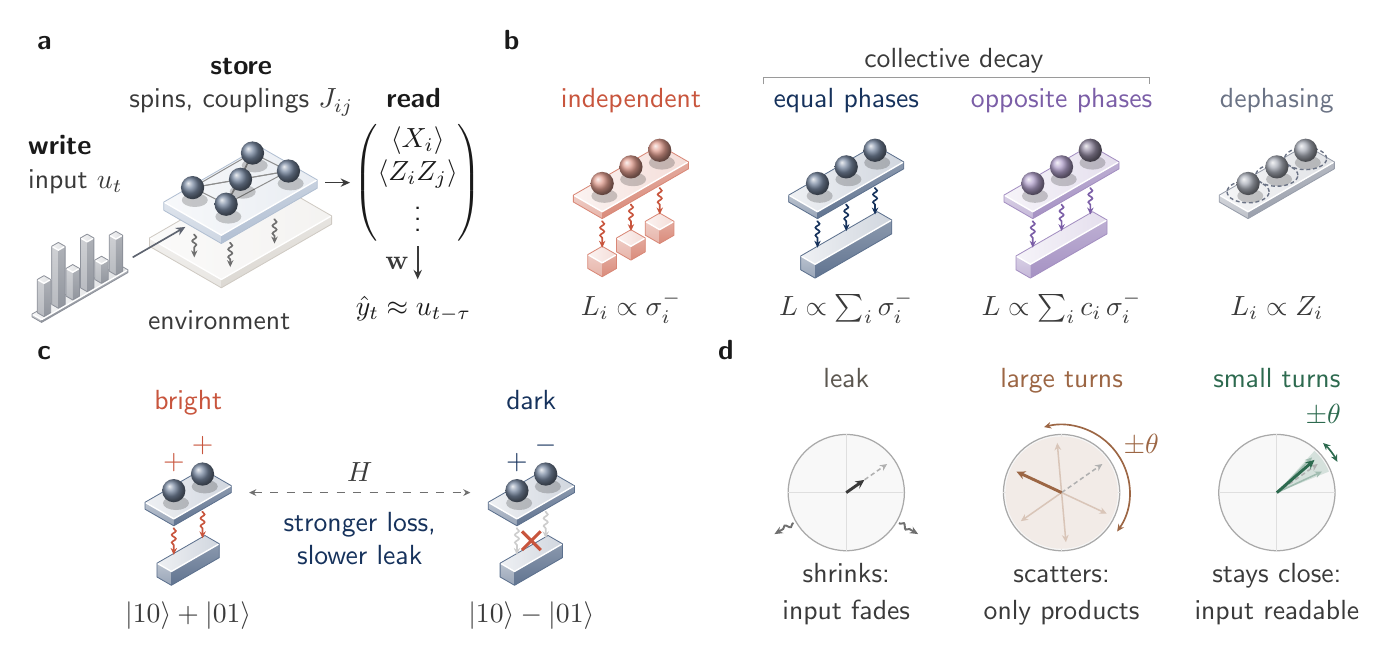
\begin{tikzpicture}[x=1pt,y=1pt,
  font=\fontsize{10}{12}\selectfont, text=ink,
  ttl/.style={anchor=base west,font=\fontsize{10}{12}\selectfont\bfseries},
  head/.style={anchor=base,font=\fontsize{10}{12}\selectfont},
  lab/.style={anchor=base,inner sep=0pt},
  iso/.style={x={(0.8660pt,-0.5pt)},y={(0.8660pt,0.5pt)},z={(0pt,1pt)}},
  wavy/.style={-{Stealth[length=2.5pt,width=2.3pt]},#1,line width=0.6pt,decorate,
    decoration={snake,amplitude=0.75pt,segment length=2.8pt,pre length=0.3pt,post length=2.4pt}},
  wavy/.default=ink3,
  decay/.style={-{Stealth[length=3pt,width=2.6pt]},#1,line width=0.7pt,
    decorate,decoration={snake,amplitude=0.85pt,segment length=3.4pt,pre length=0.5pt,post length=2.4pt}},
  arr/.style={-{Stealth[length=3.4pt,width=3pt]},ink2,line width=0.6pt},
  lvl/.style={line width=1.2pt,line cap=round,#1},
  mix/.style={{Stealth[length=2.6pt,width=2.4pt]}-{Stealth[length=2.6pt,width=2.4pt]},ink3,dashed,line width=0.5pt},
]
\path[use as bounding box] (0,0) rectangle (483.7,218);

% isometric boxes from (#1,#2,#3) to (#4,#5,#6) in colour #7: the three faces that face the viewer, lit from the
% upper left; \isopale is the same, paler, for the environment
\newcommand{\isobox}[7]{%
  \shade[top color=#7!30,bottom color=#7!44] (#1,#2,#3) -- (#4,#2,#3) -- (#4,#2,#6) -- (#1,#2,#6) -- cycle;
  \shade[top color=#7!50,bottom color=#7!68] (#4,#2,#3) -- (#4,#5,#3) -- (#4,#5,#6) -- (#4,#2,#6) -- cycle;
  \shade[left color=#7!7,right color=#7!20] (#1,#2,#6) -- (#4,#2,#6) -- (#4,#5,#6) -- (#1,#5,#6) -- cycle;
  \draw[white,line width=0.5pt,line join=round,line cap=round] (#1,#2,#6) -- (#4,#2,#6) -- (#4,#5,#6);
  \draw[#7!70,line width=0.3pt,line join=round] (#1,#2,#3) -- (#4,#2,#3) -- (#4,#5,#3) -- (#4,#5,#6) -- (#1,#5,#6)
    -- (#1,#2,#6) -- cycle;}
\newcommand{\isopale}[7]{%
  \shade[top color=#7!16,bottom color=#7!26] (#1,#2,#3) -- (#4,#2,#3) -- (#4,#2,#6) -- (#1,#2,#6) -- cycle;
  \shade[top color=#7!28,bottom color=#7!40] (#4,#2,#3) -- (#4,#5,#3) -- (#4,#5,#6) -- (#4,#2,#6) -- cycle;
  \shade[left color=#7!5,right color=#7!13] (#1,#2,#6) -- (#4,#2,#6) -- (#4,#5,#6) -- (#1,#5,#6) -- cycle;
  \draw[white,line width=0.5pt,line join=round,line cap=round] (#1,#2,#6) -- (#4,#2,#6) -- (#4,#5,#6);
  \draw[#7!55,line width=0.3pt,line join=round] (#1,#2,#3) -- (#4,#2,#3) -- (#4,#5,#3) -- (#4,#5,#6) -- (#1,#5,#6)
    -- (#1,#2,#6) -- cycle;}
% a sphere of radius 4.2 resting on the point #1, in colour #2, with its contact shadow
\newcommand{\ball}[2]{%
  \fill[black,opacity=0.20] ($#1+(0.8,-0.3)$) ellipse (4.7pt and 2.5pt);
  \shade[ball color=#2!58!white] ($#1+(0,4.2)$) circle (4.2pt);}

\begin{scope}[yshift=106pt]
%=================================================================== a  the reservoir
\node[ttl] at (0,104) {a};
\begin{scope}[shift={(49.2pt,46pt)},iso]
  % the environment: a basin under the reservoir
  \isopale{-3}{-3}{-13}{27}{43}{-10}{env}
  % input: one bar per time step, marching into the reservoir
  \isobox{10}{-65}{-1}{14}{-29}{0}{drive}
  \foreach \yy/\h in {-32/13,-38/7,-44/18,-50/10,-56/21,-62/12}{\isobox{10.6}{\yy-1.4}{0}{13.4}{\yy+1.4}{\h}{drive}}
  \coordinate (i1) at (12,-25,1.5); \coordinate (i2) at (12,-3,1.5);
  % the reservoir: a glass plate carrying five spins
  \isobox{0}{0}{0}{24}{40}{3}{glass}
  \foreach \k/\px/\py in {1/5/32,2/19/33,3/12/20,4/5/7,5/18/8}{\coordinate (f\k) at (\px,\py,3);}
\end{scope}
\foreach \k in {1,...,5}{\coordinate (s\k) at ($(f\k)+(0,4.2)$);}
\foreach \i/\j in {1/2,1/3,1/4,1/5,2/3,2/4,2/5,3/4,3/5,4/5}{\draw[ink3!80,line width=0.35pt] (s\i) -- (s\j);}
\foreach \k in {1,...,5}{\ball{(f\k)}{shared}}
\draw[arr,drive] (i1) -- (i2);
\node[lab,anchor=base west,text=ink2] at (0,54) {input $u_t$};
% the three steps of a memory: write, store, read
\node[lab,anchor=base west,font=\fontsize{10}{12}\selectfont\bfseries] at (0,66) {write};
\node[lab,font=\fontsize{10}{12}\selectfont\bfseries] at (77.2,95) {store};
\node[lab,font=\fontsize{10}{12}\selectfont\bfseries] at (139.5,83) {read};
\node[lab,text=ink2] at (77.2,83) {spins, couplings $J_{ij}$};
\draw[wavy] (60.2,37.5) -- (60.2,29);
\draw[wavy] (73.2,34.5) -- (73.2,25.5);
\draw[wavy] (89.2,43) -- (89.2,34);
\node[lab,text=ink2] at (69.2,3) {environment};
% linear readout
\draw[arr] (107.5,56) -- (116.5,56);
\node[anchor=west,inner sep=0pt] (x) at (117.5,56)
  {$\begin{pmatrix}\langle X_i\rangle\\ \langle Z_iZ_j\rangle\\ \vdots\end{pmatrix}$};
\draw[arr] ($(x.south)+(0,-1.5)$) -- ++(0,-12);
\node[lab,anchor=base east,text=ink2] at ($(x.south)+(-3,-10)$) {$\mathbf w$};
\node[lab,anchor=base east] at (160.5,8) {$\hat y_t\approx u_{t-\tau}$};

%=================================================================== b  the shapes of the environment
\node[ttl] at (168.5,104) {b};
% a glass tile with three spins, centred at x = #1, tinted #2; the baths are drawn before it
\newcommand{\tile}[2]{%
  \begin{scope}[shift={(#1pt-20.8pt,49pt)},iso]
    \isobox{0}{0}{0}{12}{36}{2.5}{#2}
    \foreach \k/\py in {1/6,2/18,3/30}{\coordinate (t\k) at (6,\py,2.5);}
  \end{scope}}
\newcommand{\spheres}[1]{\foreach \k in {3,2,1}{\ball{(t\k)}{#1}}}
% baths under the tile: one for each spin, or one for all
\newcommand{\cubes}[2]{%
  \begin{scope}[shift={(#1pt-20.8pt,49pt)},iso]
    \foreach \py in {30,18,6}{\isobox{3}{\py-3}{-24}{9}{\py+3}{-19}{#2}}
  \end{scope}}
\newcommand{\slabbath}[2]{%
  \begin{scope}[shift={(#1pt-20.8pt,49pt)},iso]\isobox{3}{2}{-24}{9}{34}{-19}{#2}\end{scope}}
% decays from under the tile into the baths
\newcommand{\drops}[2]{%
  \draw[wavy=#2] (#1-10.4,42.3) -- (#1-10.4,32.5);
  \draw[wavy=#2] (#1,48.3) -- (#1,38.5);
  \draw[wavy=#2] (#1+10.4,54.3) -- (#1+10.4,44.5);}
\newcommand{\jumps}[2]{\node[lab,text=ink2] at (#1,8) {#2};}
% four columns 77.8 pt apart, the first as far from panel a as they are from each other; the last three
% stand above the three columns of panel d
% local
\node[lab,text=local] at (218.0,83) {independent};
\cubes{218.0}{local}\drops{218.0}{local}\tile{218.0}{local}\spheres{local}
\jumps{218.0}{$L_i\propto\sigma_i^-$}
% one shared channel, equal phases; a bracket joins it with the next column as collective decay
\node[lab,text=shared] at (295.8,83) {equal phases};
\draw[ink3!70,line width=0.45pt] (266,91.5) -- (266,94) -- (405.4,94) -- (405.4,91.5);
\node[lab,text=ink2] at (334.7,97.5) {collective decay};
\slabbath{295.8}{shared}\drops{295.8}{shared}\tile{295.8}{shared}\spheres{shared}
\jumps{295.8}{$L\propto\sum_i\sigma_i^-$}
% the same channel with opposite phases: the darker spin decays with the reversed phase
\node[lab,text=opp] at (373.6,83) {opposite phases};
\slabbath{373.6}{opp}\drops{373.6}{opp}\tile{373.6}{opp}
\ball{(t3)}{opp!55!black}\ball{(t2)}{opp}\ball{(t1)}{opp}
\jumps{373.6}{$L\propto\sum_ic_i\,\sigma_i^-$}
% dephasing: rings of random phase around each spin; no bath takes energy
\node[lab,text=deph] at (451.4,83) {dephasing};
\tile{451.4}{deph}
\foreach \k in {3,2,1}{
  \draw[deph,line width=0.5pt,dash pattern=on 1.4pt off 1pt] ($(t\k)+(0,1.2)$) ++(7.6,0)
     arc[start angle=0,end angle=180,x radius=7.6pt,y radius=4.0pt];
  \ball{(t\k)}{deph}
  \draw[deph,line width=0.5pt,dash pattern=on 1.4pt off 1pt] ($(t\k)+(0,1.2)$) ++(-7.6,0)
     arc[start angle=180,end angle=360,x radius=7.6pt,y radius=4.0pt];}
\jumps{451.4}{$L_i\propto Z_i$}
\end{scope}

%=================================================================== c  bright and dark states
\node[ttl] at (0,98) {c};
% two spins with one excitation on a glass tile above one shared channel, drawn as in panel b; the tile is centred at
% x = #1 with its front corner at height #2, and its spins are named #3a (front) and #3b (back)
\newcommand{\pairslab}[2]{%
  \begin{scope}[shift={(#1pt-15.6pt,#2pt)},iso]\isobox{3}{2}{-24}{9}{22}{-19}{shared}\end{scope}}
\newcommand{\pairtile}[3]{%
  \begin{scope}[shift={(#1pt-15.6pt,#2pt)},iso]
    \isobox{0}{0}{0}{12}{24}{2.5}{shared}
    \coordinate (#3a) at (6,6,2.5); \coordinate (#3b) at (6,18,2.5);
  \end{scope}}
% bright: the excitation sits on both spins with the same sign, and their decays add
\node[lab,text=local] at (58,80) {bright};
\pairslab{58}{44}
\draw[wavy=local] (52.8,37.3) -- (52.8,27.5);
\draw[wavy=local] (63.2,43.3) -- (63.2,33.5);
\pairtile{58}{44}{B}
\ball{(Bb)}{shared}\ball{(Ba)}{shared}
\node[lab,text=local] at ($(Ba)+(0,12)$) {$+$};
\node[lab,text=local] at ($(Bb)+(0,12)$) {$+$};
\node[lab,text=ink2] at (58,3) {$|10\rangle+|01\rangle$};
% dark: opposite signs, the decays cancel and nothing reaches the channel
\node[lab,text=shared] at (182,80) {dark};
\pairslab{182}{44}
\draw[wavy=ink3!35] (176.8,37.3) -- (176.8,27.5);
\draw[wavy=ink3!35] (187.2,43.3) -- (187.2,33.5);
\draw[local,line width=1.1pt] (178.6,29.2) -- (185.4,36) (178.6,36) -- (185.4,29.2);
\pairtile{182}{44}{D}
\ball{(Db)}{shared}\ball{(Da)}{shared}
\node[lab,text=shared] at ($(Da)+(0,12)$) {$+$};
\node[lab,text=shared] at ($(Db)+(0,12)$) {$-$};
\node[lab,text=ink2] at (182,3) {$|10\rangle-|01\rangle$};
% the Hamiltonian mixes the two, so the dark state leaks through the bright one, and strong loss slows this leak
\draw[mix] (80,50) -- (160,50);
\node[lab,text=ink2] at (120,54) {$H$};
\node[lab,text=shared] at (120,36) {stronger loss,};
\node[lab,text=shared] at (120,24) {slower leak};

%=================================================================== d  two ways to forget
\node[ttl] at (246,98) {d};
\newcommand{\dial}[1]{%
  \fill[ink3!5] #1 circle (21pt);
  \draw[ink3!60,line width=0.45pt] #1 circle (21pt);
  \draw[ink3!22,line width=0.35pt] ($#1+(-21pt,0)$) -- ($#1+(21pt,0)$) ($#1+(0,-21pt)$) -- ($#1+(0,21pt)$);}
% the record of one input is an arrow, dashed where it was written; a double arc marks the turn of one later input
\tikzset{vec/.style={-{Stealth[length=2.6pt,width=2.4pt]},line width=0.55pt},
         bold/.style={-{Stealth[length=3.2pt,width=3pt]},line width=1.05pt},
         ghost/.style={-{Stealth[length=2.6pt,width=2.4pt]},ink3!55,line width=0.55pt,dash pattern=on 1.6pt off 1.1pt},
         turn/.style={{Stealth[length=2.6pt,width=2.4pt]}-{Stealth[length=2.6pt,width=2.4pt]},line width=0.6pt}}
% leak: the record shrinks while the environment takes it
\node[head,text=env!55!black] at (295.8,88) {leak};
\dial{(295.8,50)}
\draw[ghost] (295.8,50) -- ++(35:18pt);
\draw[bold,ink2] (295.8,50) -- ++(35:8pt);
\draw[decay=ink3] ($(295.8,50)+(-150:22pt)$) -- ++(-150:8pt);
\draw[decay=ink3] ($(295.8,50)+(-30:22pt)$) -- ++(-30:8pt);
\node[lab,text=ink2] at (295.8,17.5) {shrinks:};
\node[lab,text=ink2] at (295.8,4) {input fades};
% large turns: later inputs scatter the record over the whole circle
\node[head,text=strong] at (373.6,88) {large turns};
\dial{(373.6,50)}
\fill[strong!13] (373.6,50) circle (20.3pt);
\foreach \a in {95,215,275,335}{\draw[vec,strong!38] (373.6,50) -- ++(\a:18pt);}
\draw[ghost] (373.6,50) -- ++(35:18pt);
\draw[bold,strong] (373.6,50) -- ++(155:18pt);
\draw[turn,strong] ($(373.6,50)+(-35:24.5pt)$) arc[start angle=-35,end angle=105,radius=24.5pt];
\node[lab,text=strong] at ($(373.6,50)+(26:32pt)$) {$\pm\theta$};
\node[lab,text=ink2] at (373.6,17.5) {scatters:};
\node[lab,text=ink2] at (373.6,4) {only products};
% small turns: the record stays close to where it was written
\node[head,text=gentle] at (451.4,88) {small turns};
\dial{(451.4,50)}
\fill[gentle!20] (451.4,50) -- ++(22:20.3pt) arc[start angle=22,end angle=48,radius=20.3pt] -- cycle;
\foreach \a in {25,45}{\draw[vec,gentle!45] (451.4,50) -- ++(\a:18pt);}
\draw[ghost] (451.4,50) -- ++(35:18pt);
\draw[bold,gentle] (451.4,50) -- ++(41:18pt);
\draw[turn,gentle] ($(451.4,50)+(27:24.5pt)$) arc[start angle=27,end angle=47,radius=24.5pt];
\node[lab,text=gentle] at ($(451.4,50)+(56:30pt)$) {$\pm\theta$};
\node[lab,text=ink2] at (451.4,17.5) {stays close:};
\node[lab,text=ink2] at (451.4,4) {input readable};
\end{tikzpicture}
\end{document}
